\label{cenarioSection}
Foi feito um criador de cenários que monta um mapa distribuindo os pisos pelo cenário, é utilizado as seguintes regras da tabela \ref{cenárioRules} na geração do cenário.

\begin{table}[]
	\centering
	\begin{tabular}{ll}
		Q $\Rightarrow$   & QQ{[}Q \\ 
		{[} $\Rightarrow$ & +QQ{]} \\ 
		{]} $\Rightarrow$ & QQ+QQ  \\ 
	\end{tabular}
	\caption{Conjunto de regras do L-System}
	\label{cenárioRules}
\end{table}

Ao finalizar o TurtleAgent faz a leitura da estrutura gerada pelo LSystem e monta o mapa usando como referencia a tabela \ref{cenárioTurtle}. O cenário obtido com o axioma inicial de "QQ" com 8 gerações pode ser visto na figura \ref{cenário8Gen} e na figura \ref{cenário9Gen} apresenta um cenário gerado em 6 iterações com o axioma inicial "Q+".
\begin{table}[]
	\centering
	\begin{tabular}{ll}
		Q $\Rightarrow$   & Gera um quarto.                              \\
		+  $\Rightarrow$  & Gira a direita a um ângulo de 90º.            \\
		-  $\Rightarrow$  & Gira a esquerda a um ângulo de 90º.           \\
		{[}  $\Rightarrow$ & Salva a posição e rotação atual.             \\
		{]}  $\Rightarrow$ & Volta para a ultima posição e rotação salva.
	\end{tabular}
	\caption{Regras de interpretação do TurtleAgent.}
	\label{cenárioTurtle}
\end{table}

\begin{figure}[!h]
	\centering
	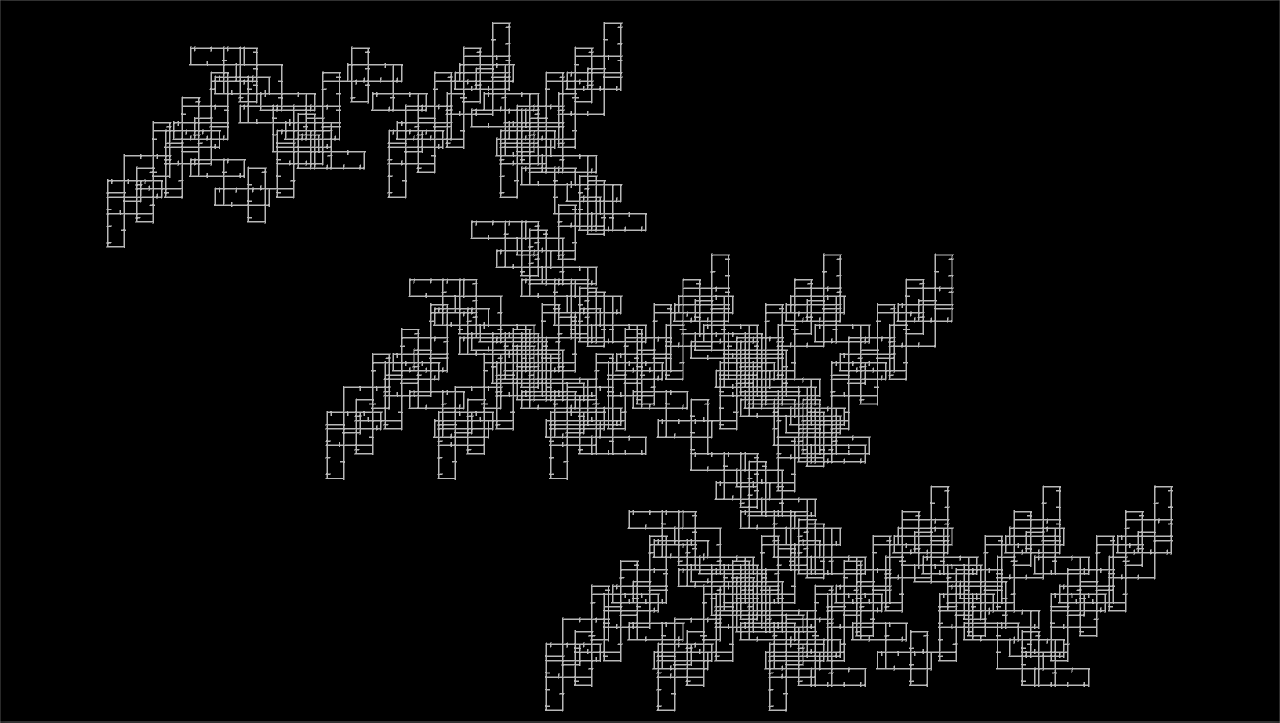
\includegraphics[width=0.4\textwidth]{Cenario2-Gen8}
	\caption{Cenário produzido na 8ª geração.}
	\label{cenário8Gen}
\end{figure}

\begin{figure}[!h]
	\centering
	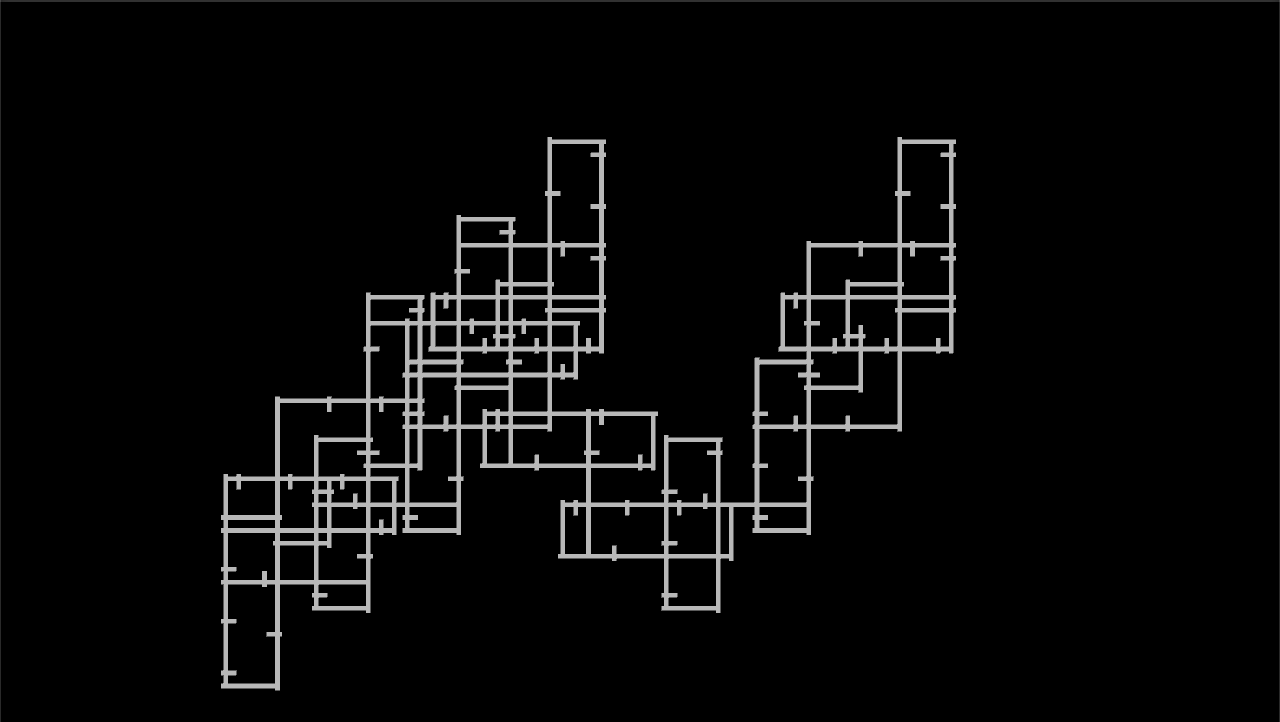
\includegraphics[width=0.4\textwidth]{Cenario3Q+-Gen6}
	\caption{Cenário produzido na 6ª geração.}
	\label{cenário9Gen}
\end{figure}

É fácil a configuração e implementação das regras usando o editor, o sistema de reescrita é bom para geração de cenários, mas necessita de algoritmos mais especializados para geração mais complexas.

\subsection{Desempenho}
Utilizando as regras de reescrita da tabela \ref{cenárioRules} na seção \ref{cenarioSection}, foi medido o tempo de execução por comprimento do axioma, definindo 15 como o numero máximo de gerações os resultados estão presentes na tabela  \ref{axiomaTempoTabela}.

\begin{table}[!h]
	\centering
	\begin{tabular}{|c|c|}
		\hline
		\textbf{Comprimento do Axioma} & \textbf{Tempo(s)} \\ \hline
		32                             & 0,0000142         \\ \hline
		124                            & 0,0000293         \\ \hline
		472                            & 0,0000917         \\ \hline
		25980                          & 0,0046719         \\ \hline
		98792                          & 0,0176053         \\ \hline
		1428512                        & 0,2621754         \\ \hline
		20655832                       & 03,7396957        \\ \hline
		78545636                       & 14,1387742        \\ \hline
		298676752*                     & 29,6070016        \\ \hline
	\end{tabular}
	\caption{Tabela com o tamanho do axioma e o tempo para ser processado em segundos. *Geração incompleta}
	\label{axiomaTempoTabela}
\end{table}

A ultima geração chegou a capacidade máxima suportada pelo stringbuilder, sua geração incompleta levou em torno de 34 segundos para ser realizada.

A figura \ref{profilerCPU} apresenta a tela do profiler na Unity sobre o uso da cpu durante os processos, aonde verifica-se a instabilidade de fps entre os processamentos, já na figura \ref{profilerMemoria} tem o uso de memoria da ferramenta durante o processamento dos axiomas, chegando até 4,80 Gb alocados na memoria.
\begin{figure}[]
	\centering
	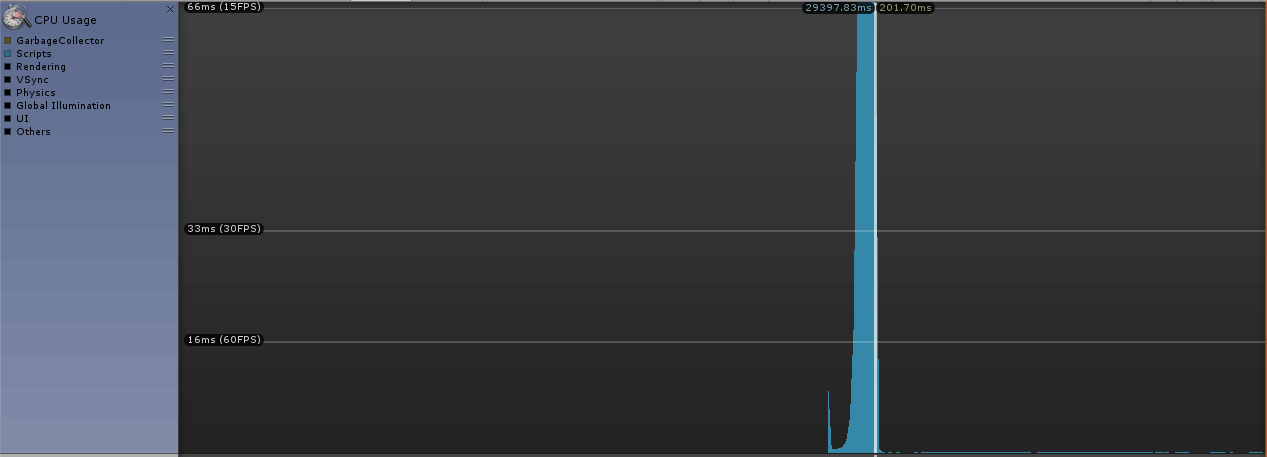
\includegraphics[width=0.45\textwidth]{Cenario-Profiler-15Gen-CPU}
	\caption{Profiler da Unity com o uso da cpu.}
	\label{profilerCPU}
\end{figure}

\begin{figure}[]
	\centering
	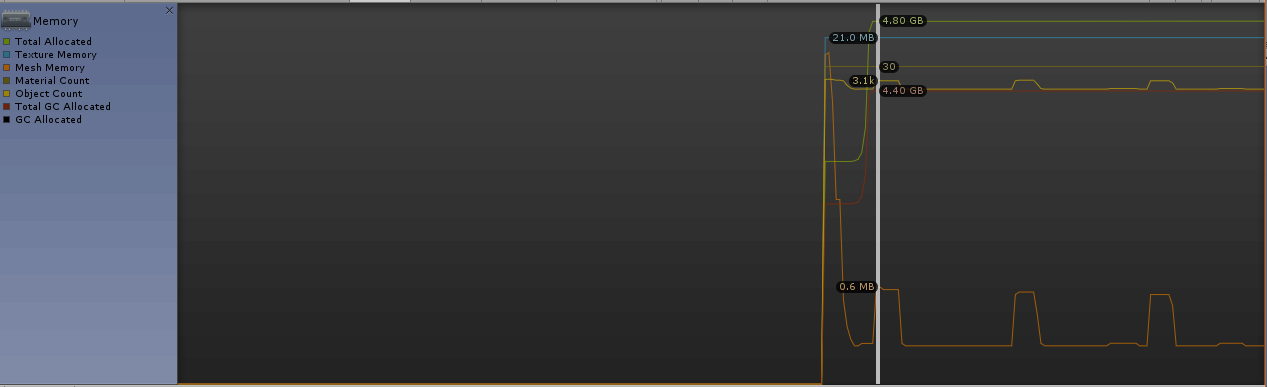
\includegraphics[width=0.45\textwidth]{Cenario-Profiler-15Gen-Memoria}
	\caption{Profiler da Unity do uso de memoria.}
	\label{profilerMemoria}
\end{figure}